\PassOptionsToPackage{unicode=true}{hyperref} % options for packages loaded elsewhere
\PassOptionsToPackage{hyphens}{url}
%
\documentclass[
  ignorenonframetext,
]{beamer}
\usepackage{pgfpages}
\setbeamertemplate{caption}[numbered]
\setbeamertemplate{caption label separator}{: }
\setbeamercolor{caption name}{fg=normal text.fg}
\beamertemplatenavigationsymbolsempty
% Prevent slide breaks in the middle of a paragraph:
\widowpenalties 1 10000
\raggedbottom
\setbeamertemplate{part page}{
  \centering
  \begin{beamercolorbox}[sep=16pt,center]{part title}
    \usebeamerfont{part title}\insertpart\par
  \end{beamercolorbox}
}
\setbeamertemplate{section page}{
  \centering
  \begin{beamercolorbox}[sep=12pt,center]{part title}
    \usebeamerfont{section title}\insertsection\par
  \end{beamercolorbox}
}
\setbeamertemplate{subsection page}{
  \centering
  \begin{beamercolorbox}[sep=8pt,center]{part title}
    \usebeamerfont{subsection title}\insertsubsection\par
  \end{beamercolorbox}
}
\AtBeginPart{
  \frame{\partpage}
}
\AtBeginSection{
  \ifbibliography
  \else
    \frame{\sectionpage}
  \fi
}
\AtBeginSubsection{
  \frame{\subsectionpage}
}
\usepackage{lmodern}
\usepackage{amssymb,amsmath}
\usepackage{ifxetex,ifluatex}
\ifnum 0\ifxetex 1\fi\ifluatex 1\fi=0 % if pdftex
  \usepackage[T1]{fontenc}
  \usepackage[utf8]{inputenc}
  \usepackage{textcomp} % provides euro and other symbols
\else % if luatex or xelatex
  \usepackage{unicode-math}
  \defaultfontfeatures{Scale=MatchLowercase}
  \defaultfontfeatures[\rmfamily]{Ligatures=TeX,Scale=1}
\fi
% use upquote if available, for straight quotes in verbatim environments
\IfFileExists{upquote.sty}{\usepackage{upquote}}{}
\IfFileExists{microtype.sty}{% use microtype if available
  \usepackage[]{microtype}
  \UseMicrotypeSet[protrusion]{basicmath} % disable protrusion for tt fonts
}{}
\makeatletter
\@ifundefined{KOMAClassName}{% if non-KOMA class
  \IfFileExists{parskip.sty}{%
    \usepackage{parskip}
  }{% else
    \setlength{\parindent}{0pt}
    \setlength{\parskip}{6pt plus 2pt minus 1pt}}
}{% if KOMA class
  \KOMAoptions{parskip=half}}
\makeatother
\usepackage{xcolor}
\IfFileExists{xurl.sty}{\usepackage{xurl}}{} % add URL line breaks if available
\IfFileExists{bookmark.sty}{\usepackage{bookmark}}{\usepackage{hyperref}}
\hypersetup{
  pdftitle={Simple \& Multiple Correspondence Analyses},
  pdfauthor={Derek Beaton},
  pdfborder={0 0 0},
  breaklinks=true}
\urlstyle{same}  % don't use monospace font for urls
\newif\ifbibliography
\usepackage{graphicx,grffile}
\makeatletter
\def\maxwidth{\ifdim\Gin@nat@width>\linewidth\linewidth\else\Gin@nat@width\fi}
\def\maxheight{\ifdim\Gin@nat@height>\textheight\textheight\else\Gin@nat@height\fi}
\makeatother
% Scale images if necessary, so that they will not overflow the page
% margins by default, and it is still possible to overwrite the defaults
% using explicit options in \includegraphics[width, height, ...]{}
\setkeys{Gin}{width=\maxwidth,height=\maxheight,keepaspectratio}
\setlength{\emergencystretch}{3em}  % prevent overfull lines
\providecommand{\tightlist}{%
  \setlength{\itemsep}{0pt}\setlength{\parskip}{0pt}}
\setcounter{secnumdepth}{-2}

% set default figure placement to htbp
\makeatletter
\def\fps@figure{htbp}
\makeatother

\usepackage{amssymb}
\usepackage{amsmath}
\usepackage{mathtools}
\usepackage{animate}
\usepackage{caption}
\captionsetup[figure]{labelformat=empty}
\usepackage{booktabs}
\usepackage{longtable}
\usepackage{array}
\usepackage{multirow}
\usepackage{wrapfig}
\usepackage{float}
\usepackage{colortbl}
\usepackage{pdflscape}
\usepackage{tabu}
\usepackage{threeparttable}
\AtBeginSubsection{}
\usepackage{textcomp}

\title{Simple \& Multiple Correspondence Analyses}
\subtitle{Contingency, categorical, ordinal, continuous and mixed data}
\author{Derek Beaton}
\date{October 27, 2019}
\institute{Rotman Research Institute}

\begin{document}
\frame{\titlepage}

\hypertarget{before-we-get-started}{%
\section{Before we get started}\label{before-we-get-started}}

\begin{frame}{Our new best friends}
\protect\hypertarget{our-new-best-friends}{}

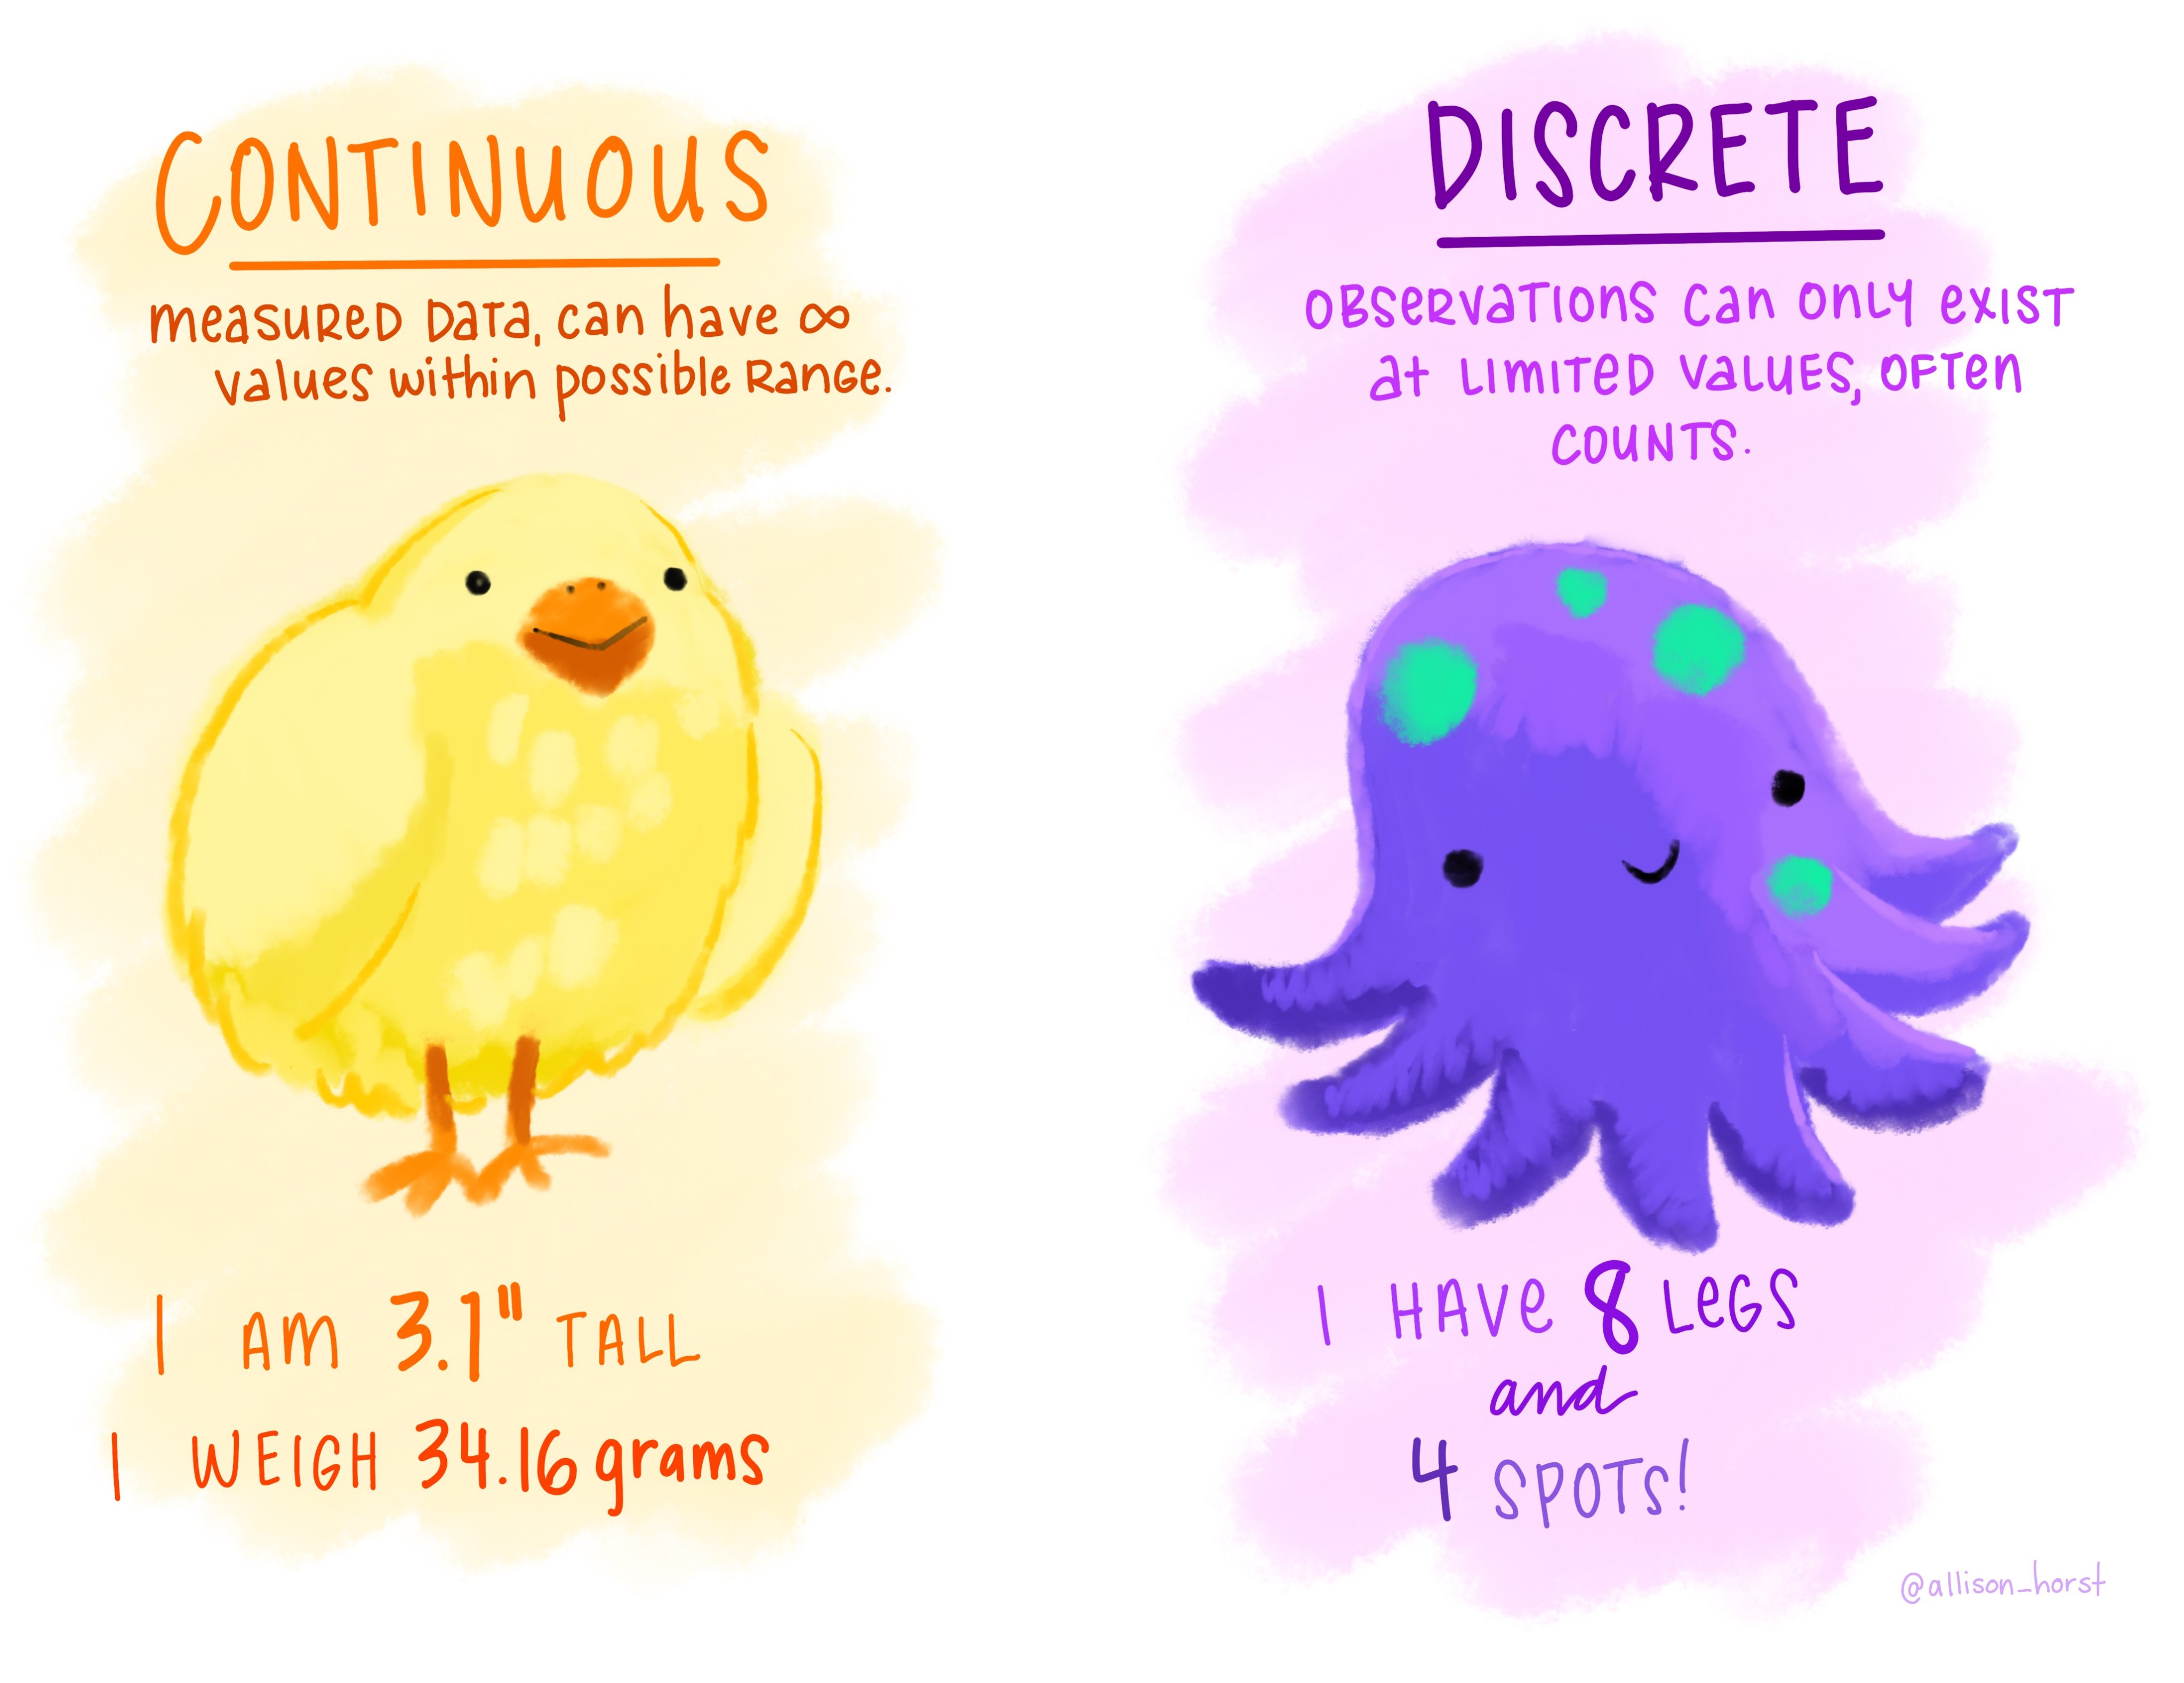
\includegraphics[width=\textwidth,height=0.75\textheight]{../images/cont_disc.jpg}

\href{https://twitter.com/allison_horst}{via @allison\_horst}

\end{frame}

\begin{frame}

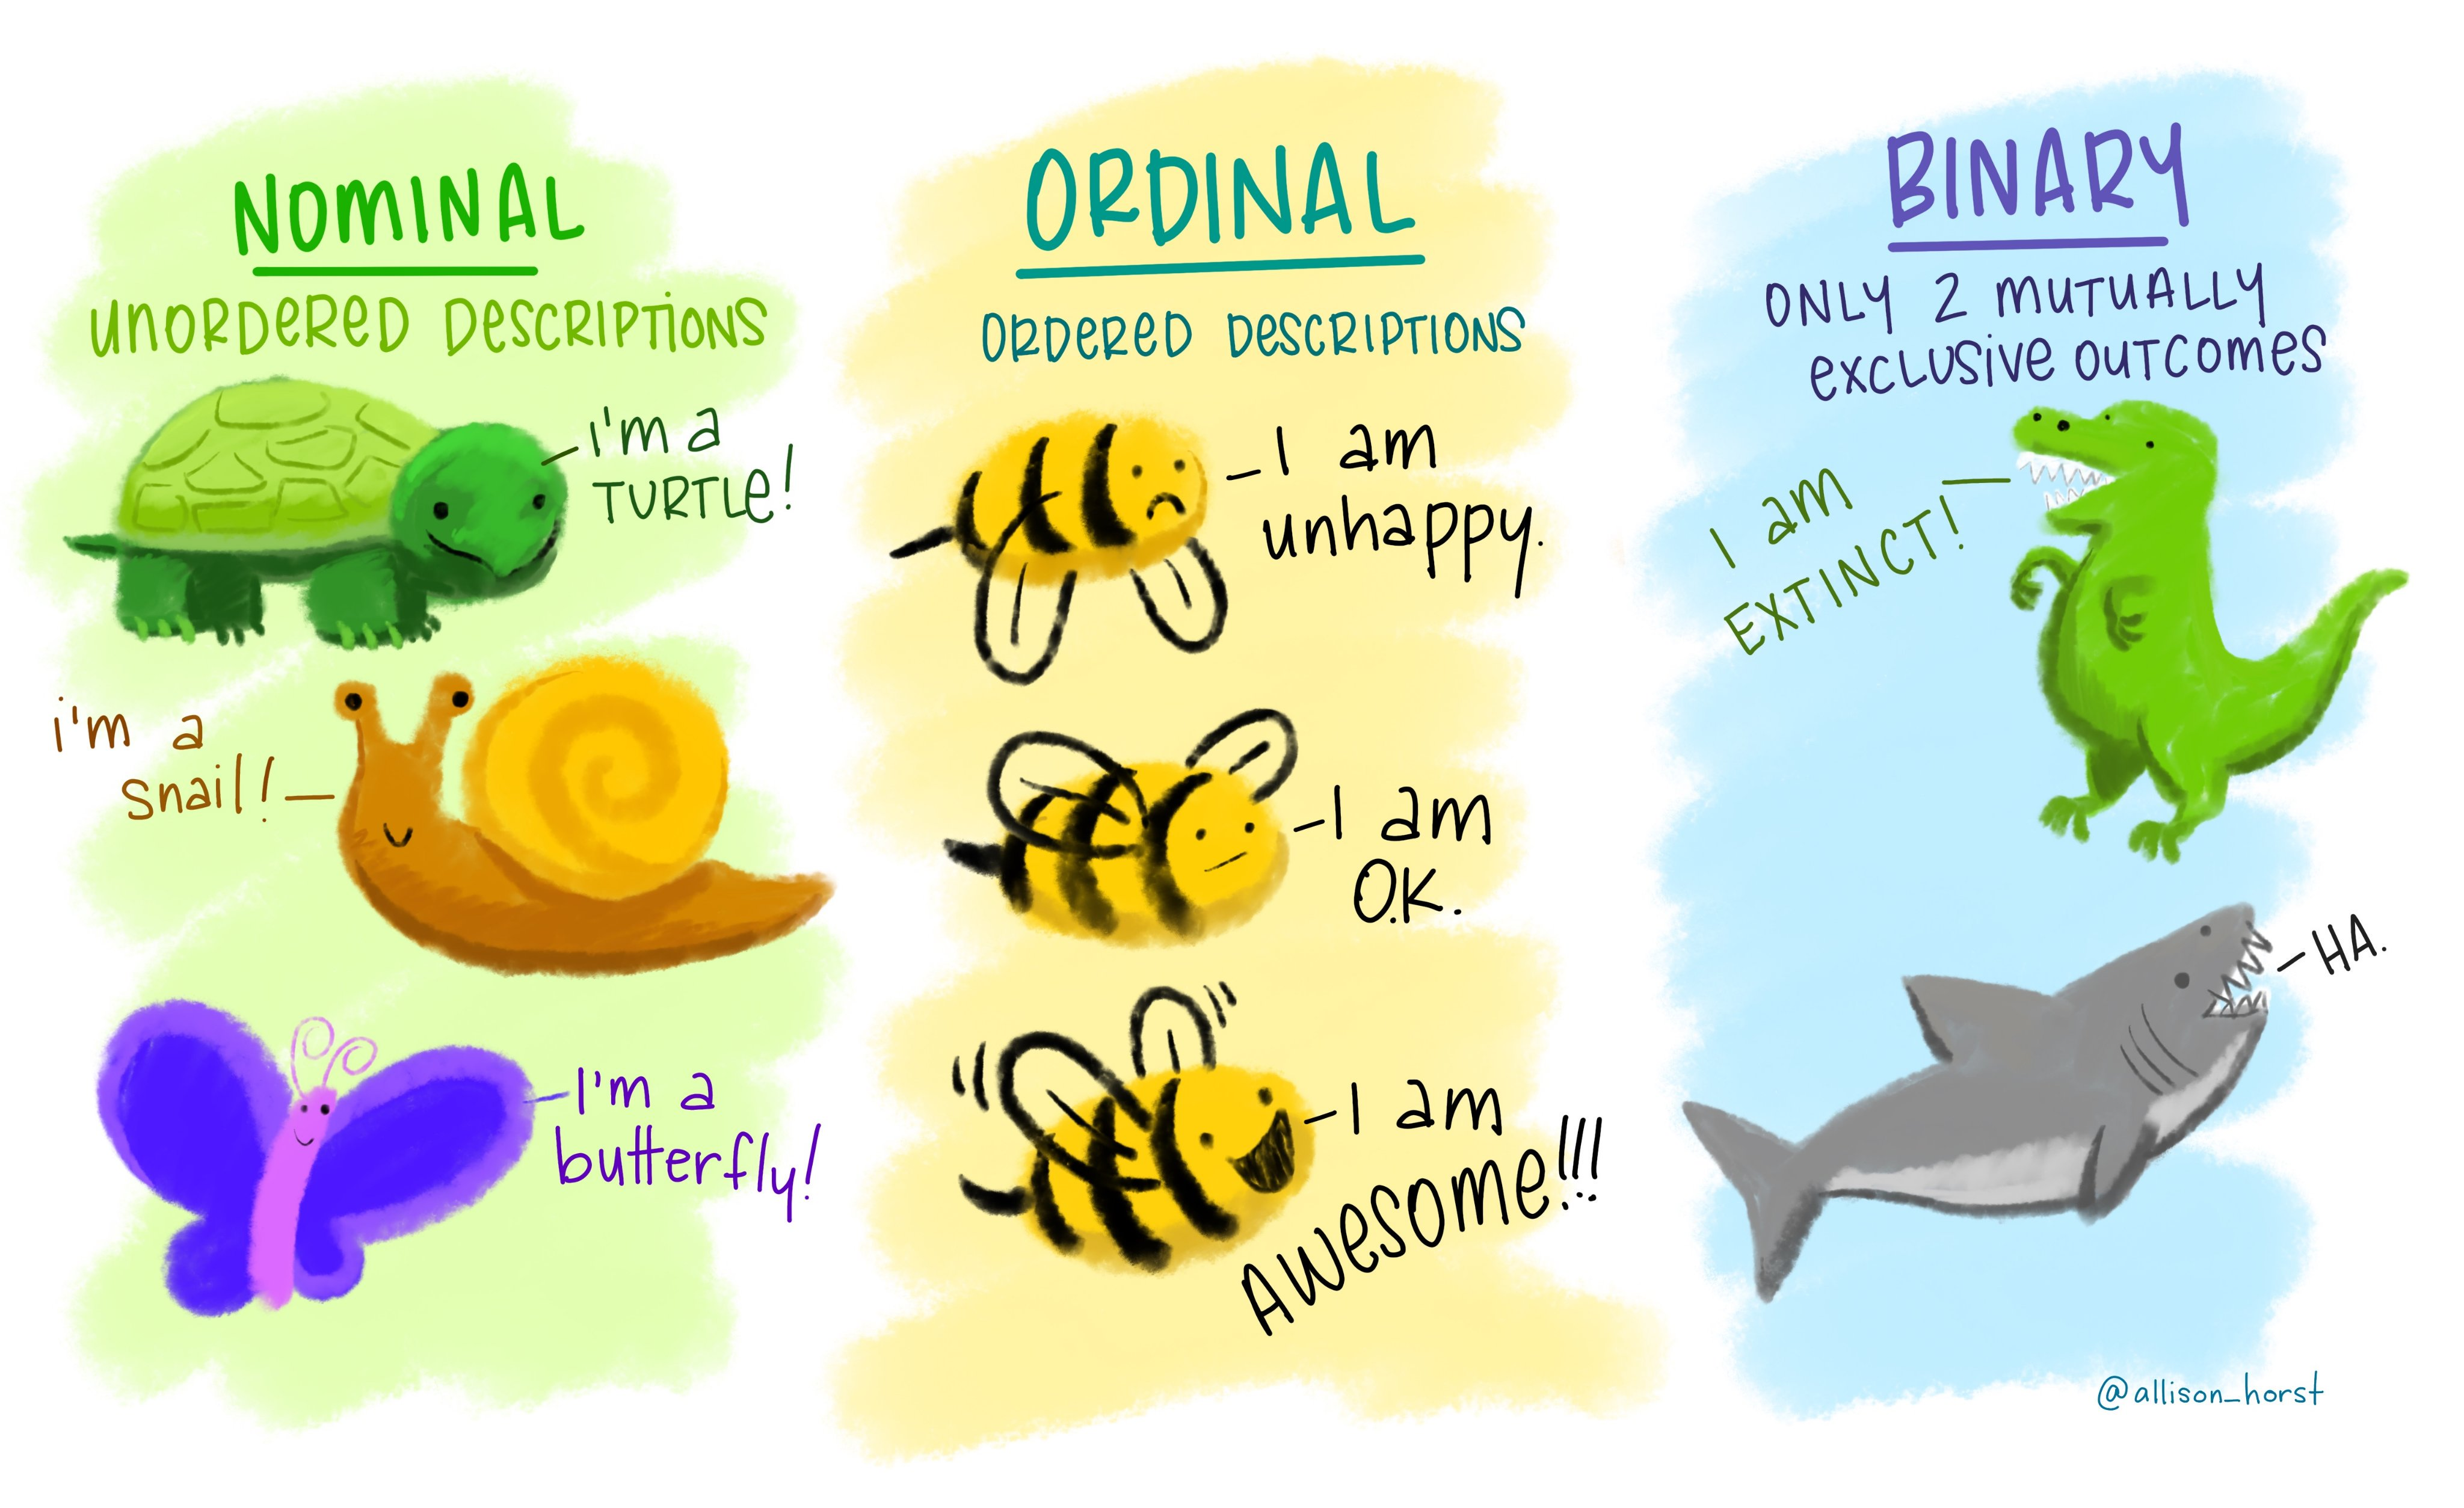
\includegraphics[width=\textwidth,height=0.75\textheight]{../images/nom_ord_bin.jpg}

\href{https://twitter.com/allison_horst}{via @allison\_horst}

\end{frame}

\begin{frame}

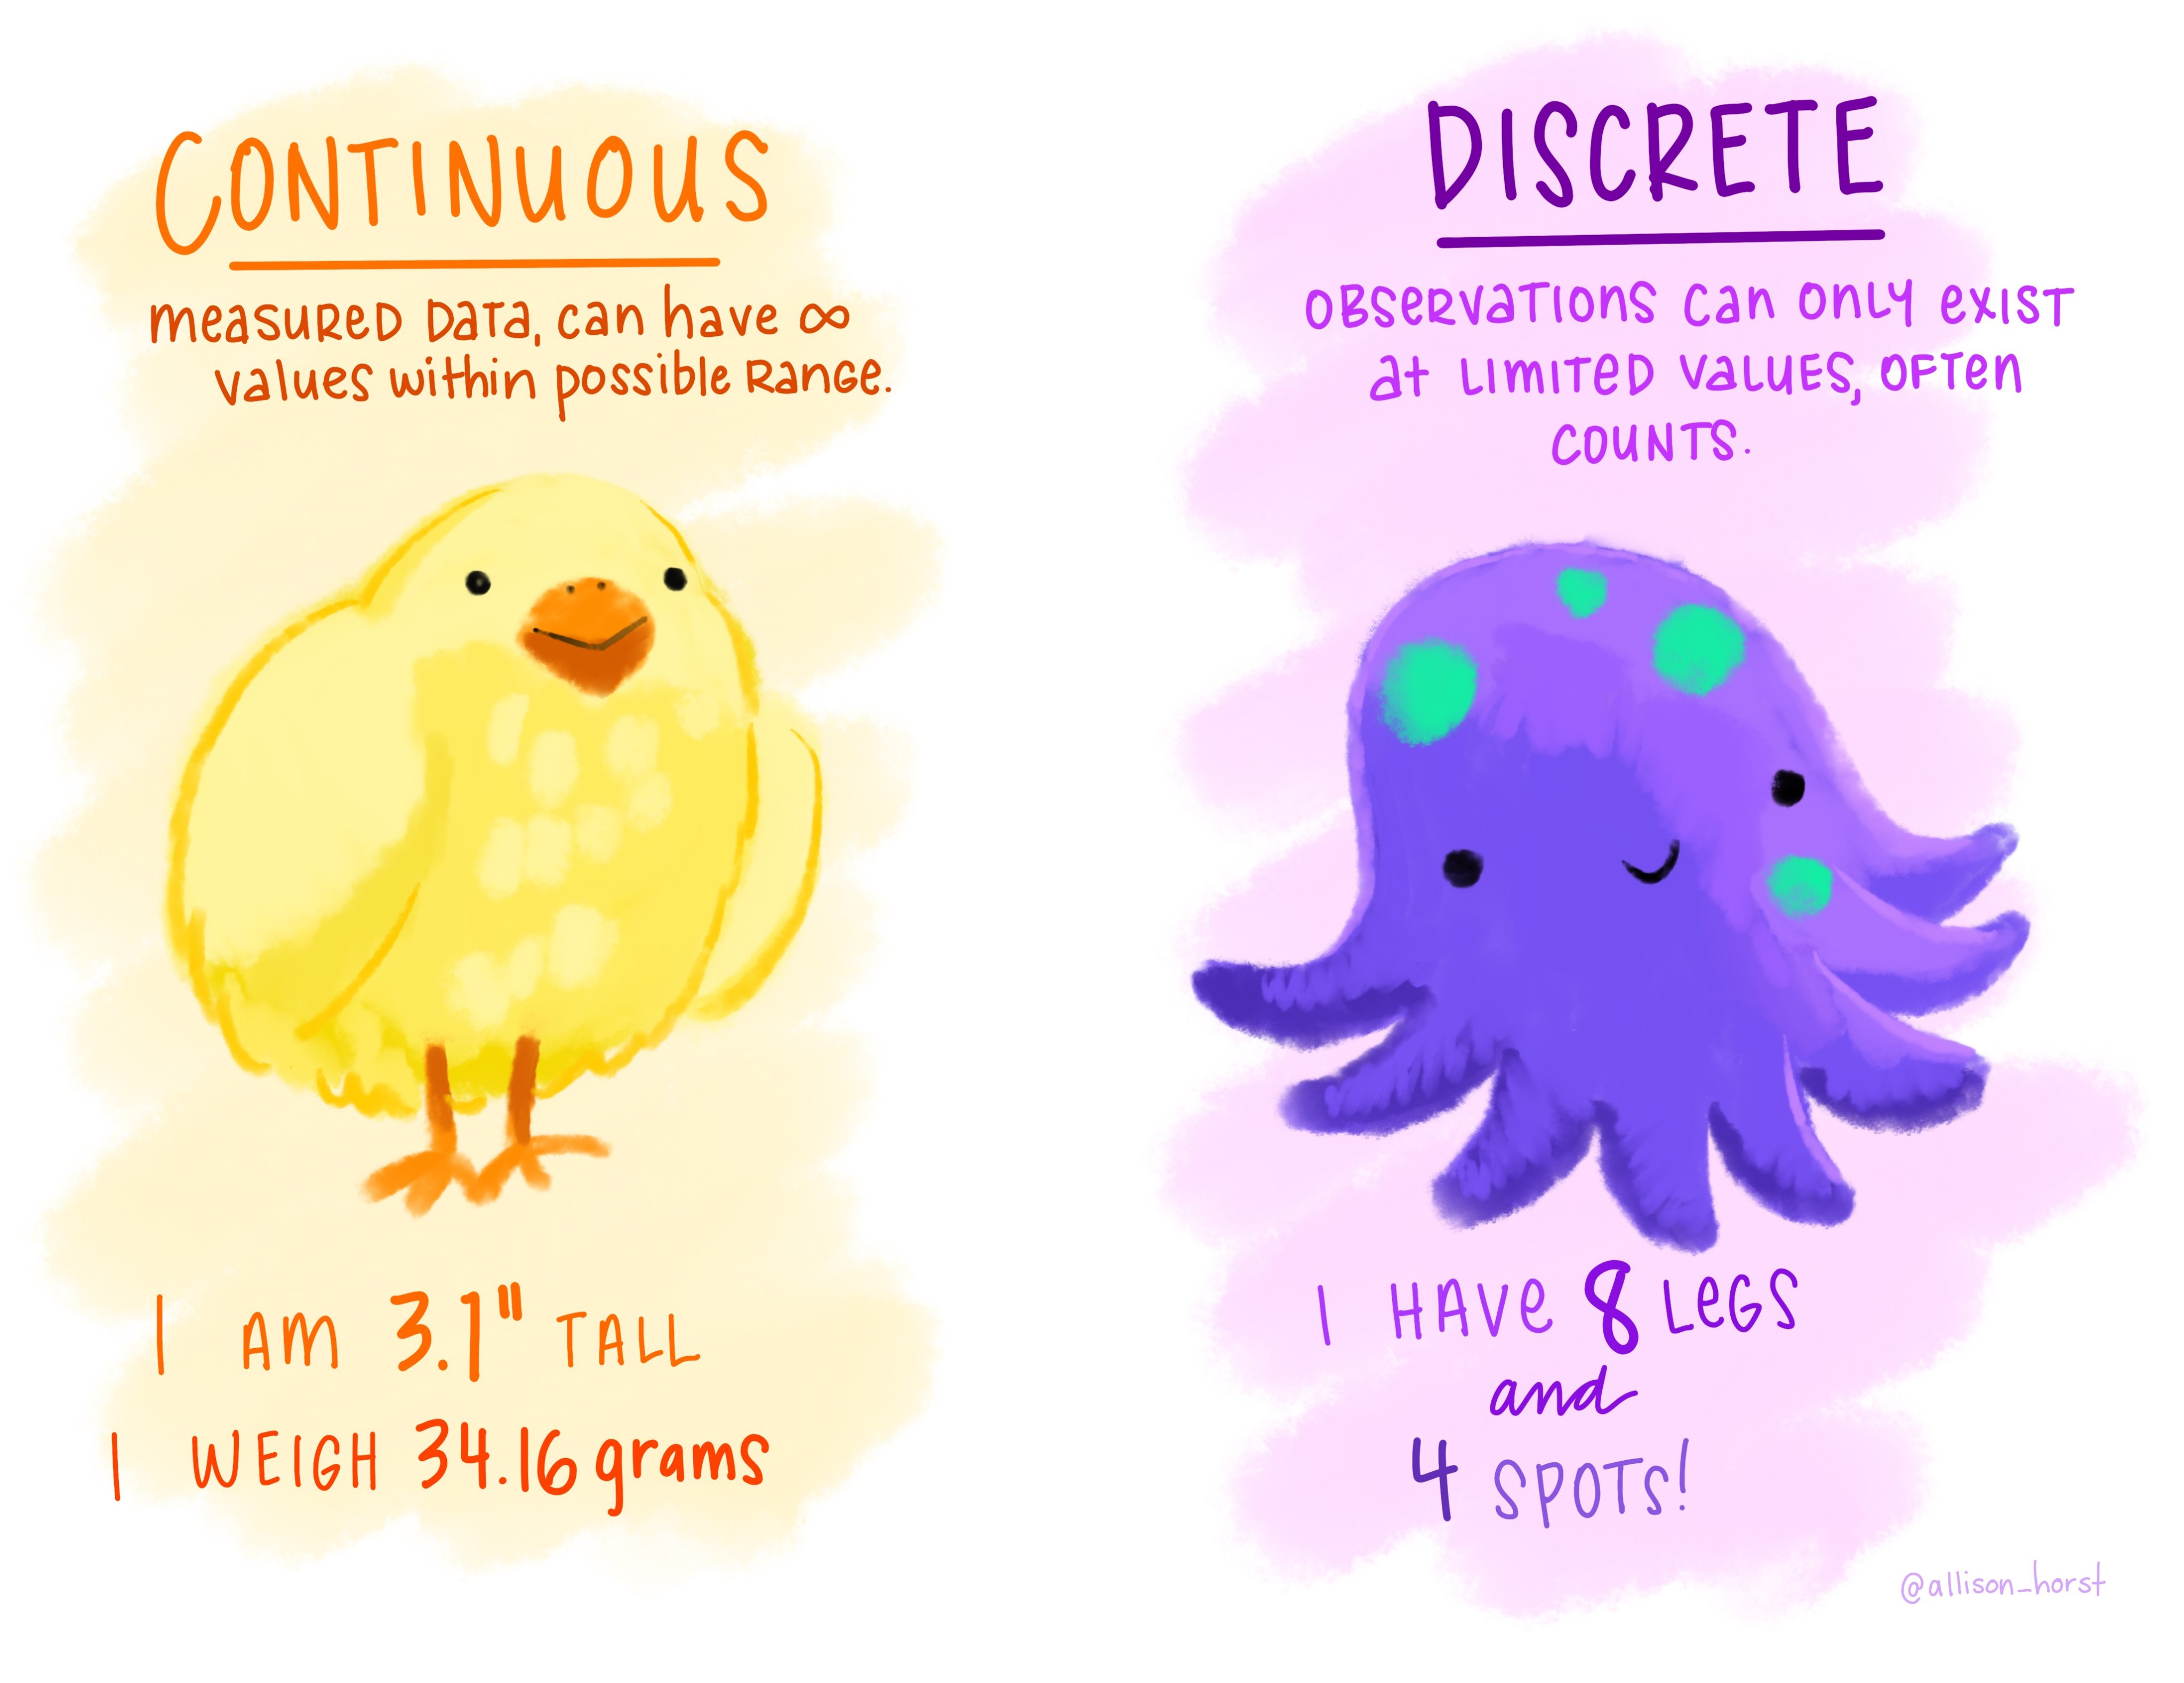
\includegraphics[width=\textwidth,height=0.4\textheight]{../images/cont_disc.jpg}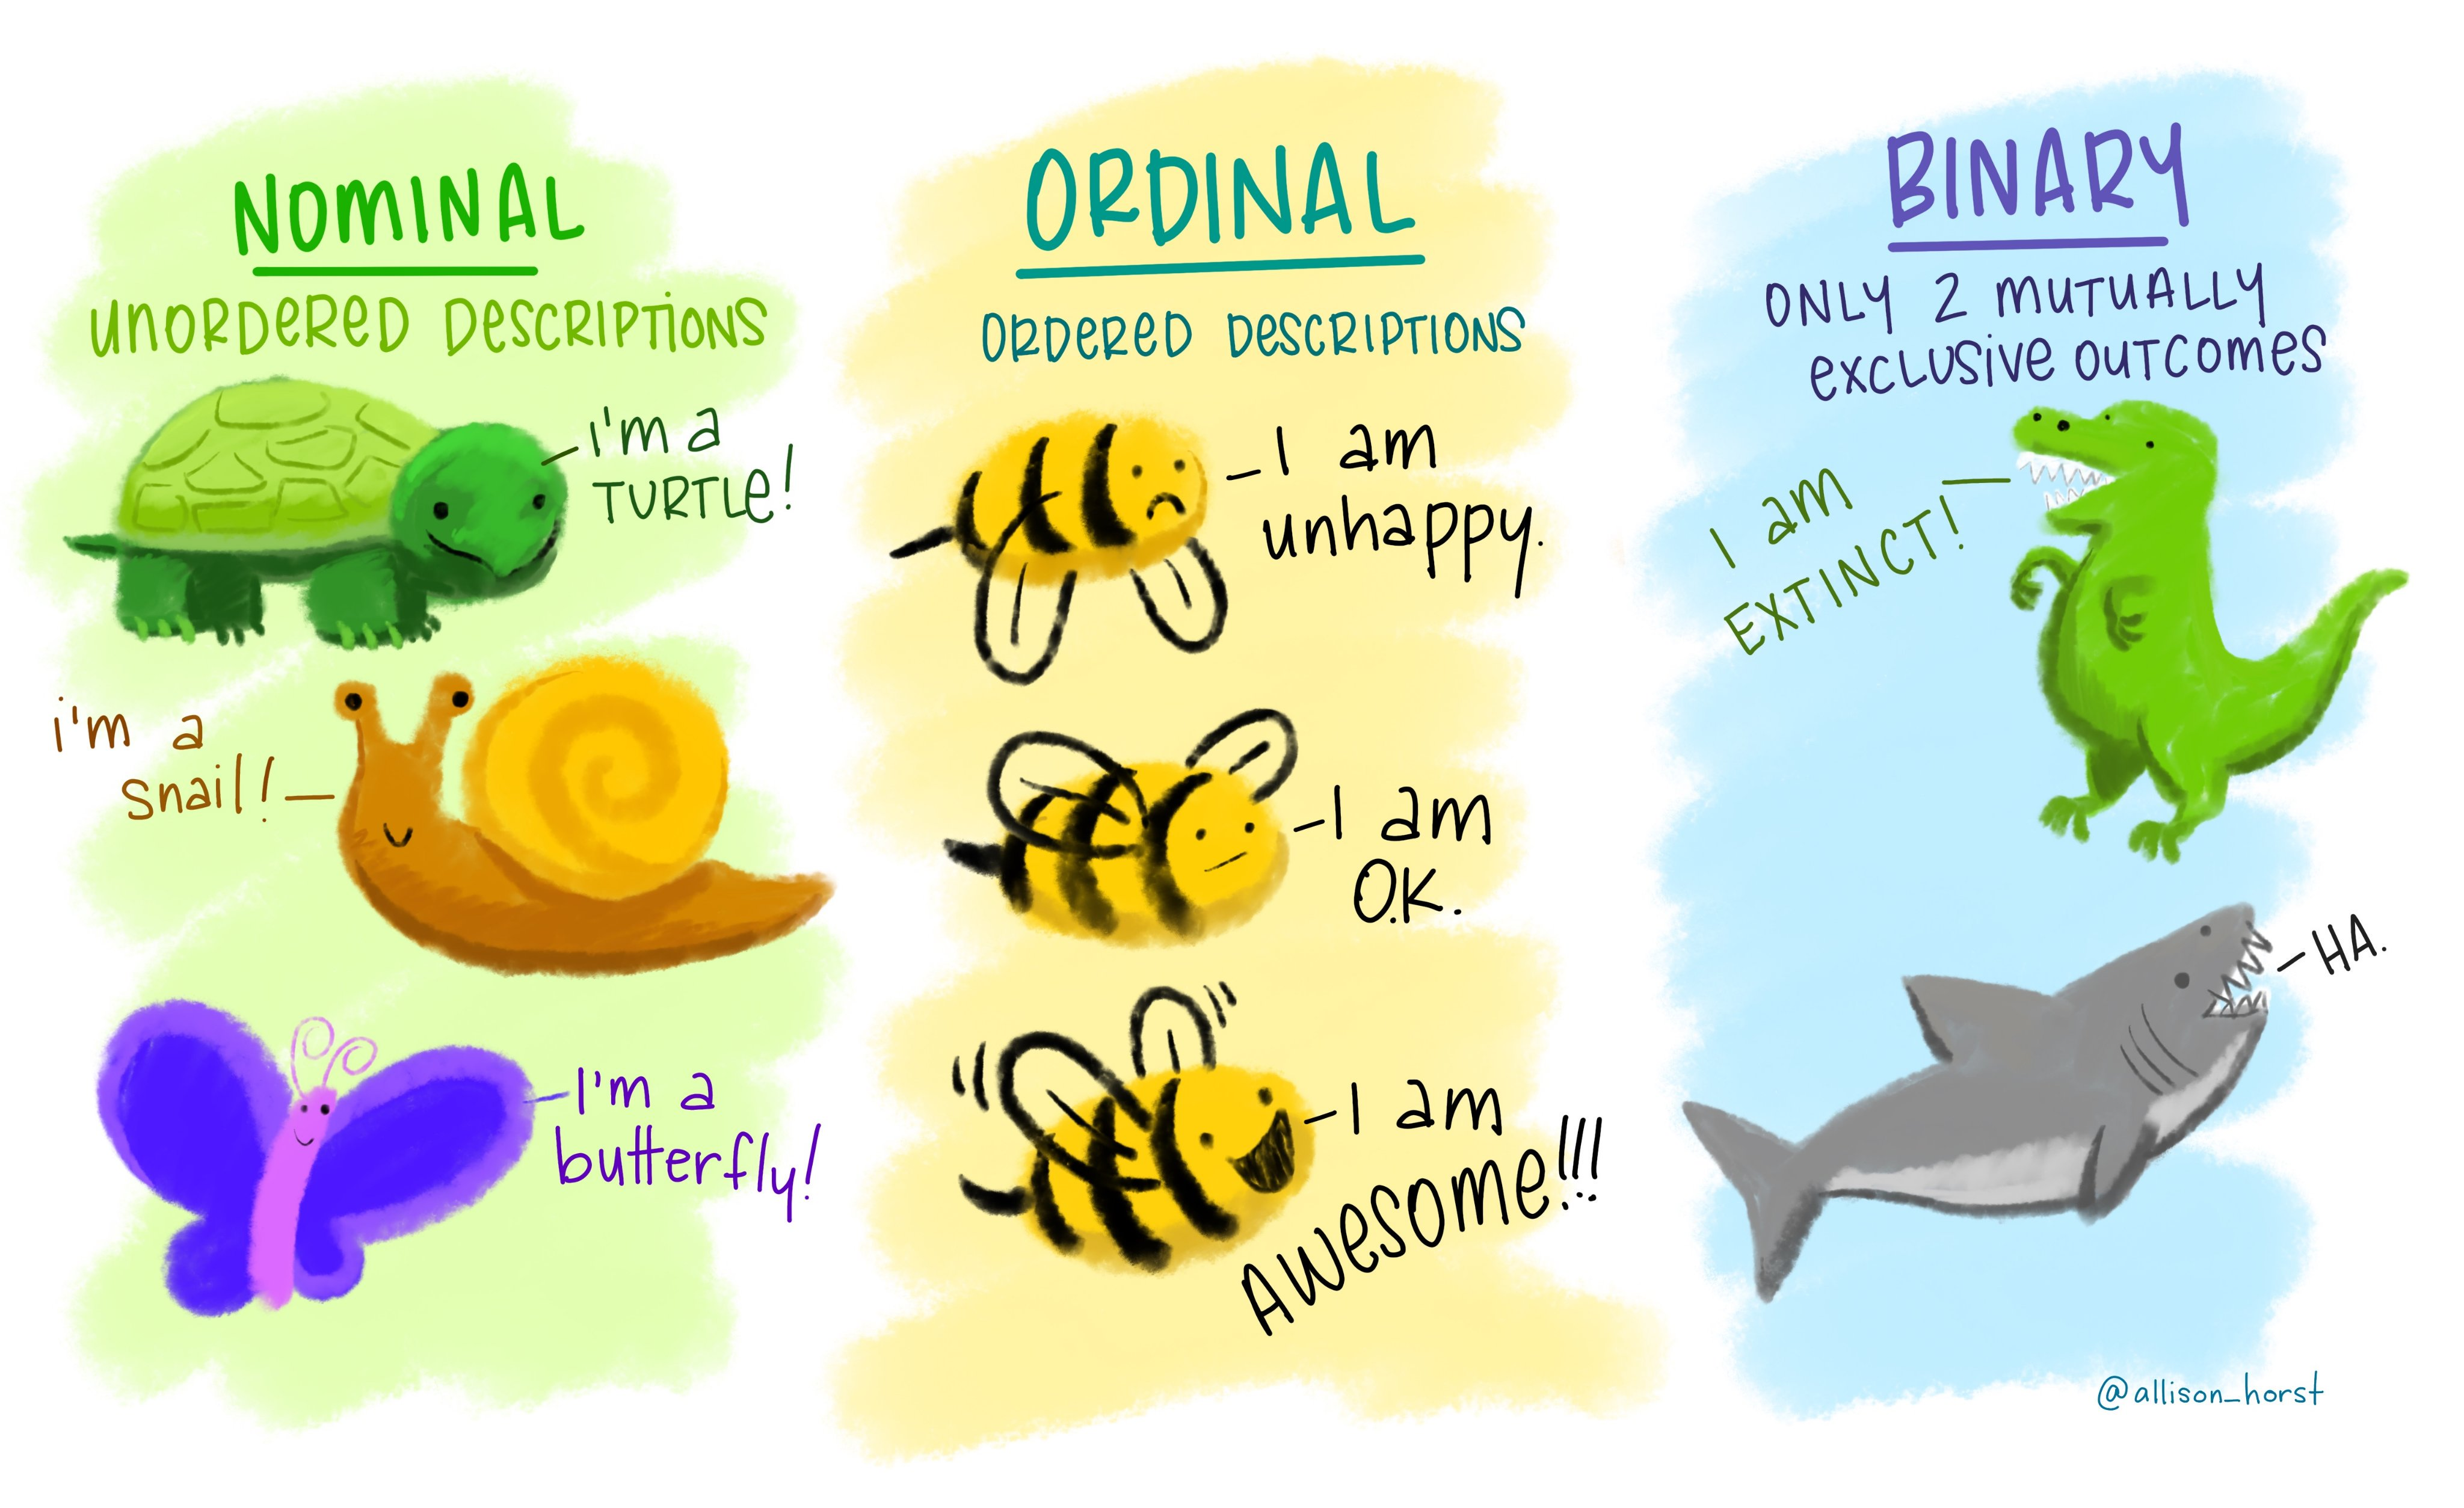
\includegraphics[width=\textwidth,height=0.4\textheight]{../images/nom_ord_bin.jpg}

\href{https://twitter.com/allison_horst}{via @allison\_horst}

\end{frame}

\begin{frame}{Motivation for today}
\protect\hypertarget{motivation-for-today}{}

\begin{itemize}[<+->]
\tightlist
\item
  Not everything is a number
\item
  Sometimes numbers aren't numbers!
\item
  We need to recognize when this happens

  \begin{itemize}[<+->]
  \tightlist
  \item
    And know what to do
  \end{itemize}
\end{itemize}

\end{frame}

\begin{frame}{Typology}
\protect\hypertarget{typology}{}

\begin{itemize}[<+->]
\tightlist
\item
  SS Stevens (not a boat!)
\item
  Levels of measurement
\item
  Excellent examples:
  \url{https://en.wikipedia.org/wiki/Level_of_measurement}
\end{itemize}

\end{frame}

\begin{frame}{Where to find everything}
\protect\hypertarget{where-to-find-everything}{}

\begin{itemize}[<+->]
\tightlist
\item
  Generally: \url{https://github.com/derekbeaton/workshops}
\item
  Today:
\end{itemize}

\end{frame}

\begin{frame}{Overview}
\protect\hypertarget{overview}{}

\begin{itemize}[<+->]
\tightlist
\item
  Revisit PCA
\item
  Looking at some data
\item
  Simple correspondence analysis

  \begin{itemize}[<+->]
  \tightlist
  \item
    and many of its connections
  \end{itemize}
\item
  Multiple correspondence analysis

  \begin{itemize}[<+->]
  \tightlist
  \item
    generalizes CA (amongst many other things)
  \item
    and how to handle various data types
  \end{itemize}
\item
  A whole bunch of bonuses

  \begin{itemize}[<+->]
  \tightlist
  \item
    Robustness
  \item
    PLS
  \item
    Networks
  \item
    Software
  \end{itemize}
\end{itemize}

\end{frame}

\hypertarget{revisting-pca}{%
\section{Revisting PCA}\label{revisting-pca}}

\begin{frame}{What is PCA for?}
\protect\hypertarget{what-is-pca-for}{}

\begin{itemize}[<+->]
\tightlist
\item
  When we can compute a covariance or correlation matrix
\item
  Break data into components

  \begin{itemize}[<+->]
  \tightlist
  \item
    Orthogonal
  \item
    Rank ordered
  \item
    Made of bits \& pieces of original measures
  \end{itemize}
\end{itemize}

\end{frame}

\begin{frame}{Eigen- and singular value decompositions}
\protect\hypertarget{eigen--and-singular-value-decompositions}{}

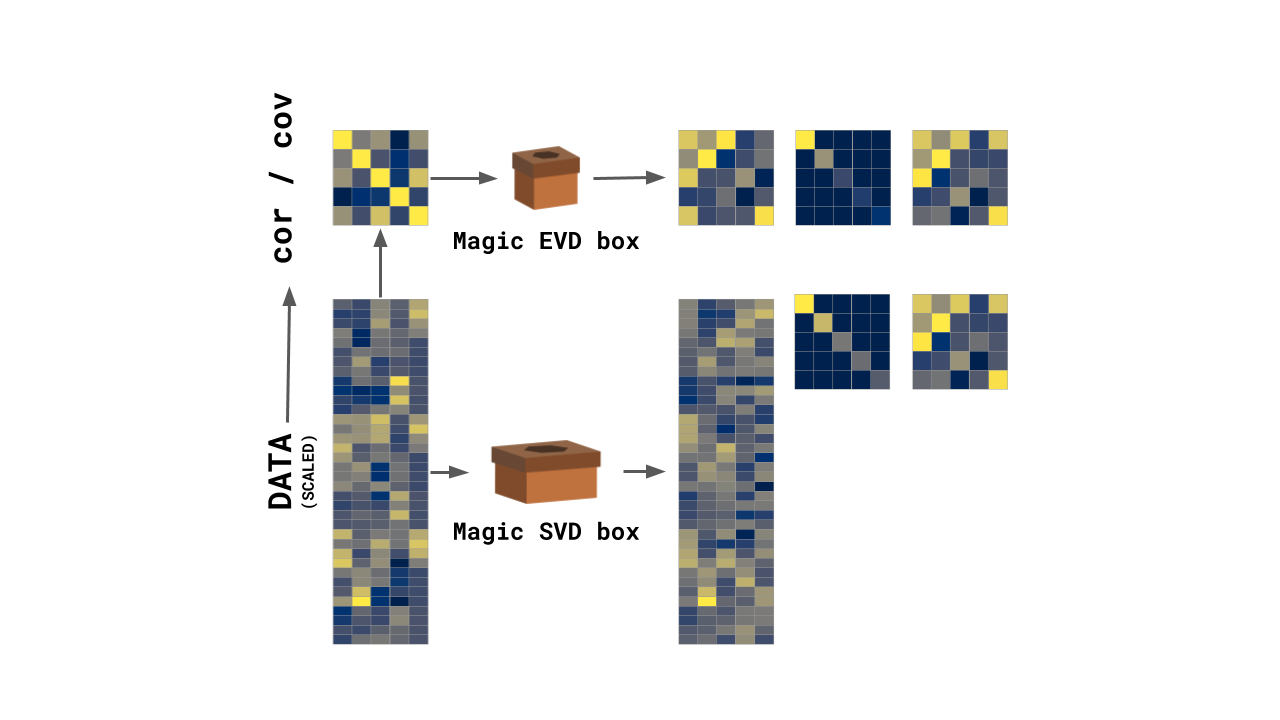
\includegraphics{../images/EVD_SVD_1.png}

\end{frame}

\begin{frame}{Eigen- and singular value decompositions}
\protect\hypertarget{eigen--and-singular-value-decompositions-1}{}

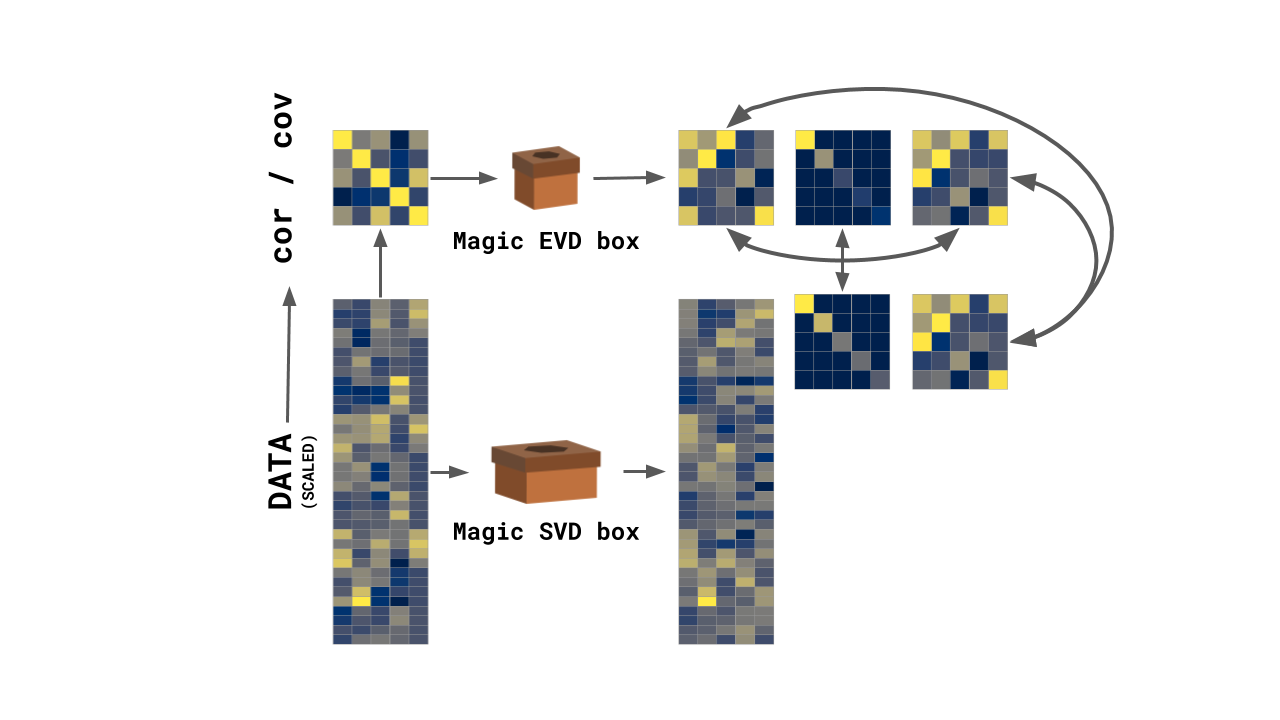
\includegraphics{../images/EVD_SVD_2.png}

\end{frame}

\begin{frame}{Eigen- and singular value decompositions}
\protect\hypertarget{eigen--and-singular-value-decompositions-2}{}

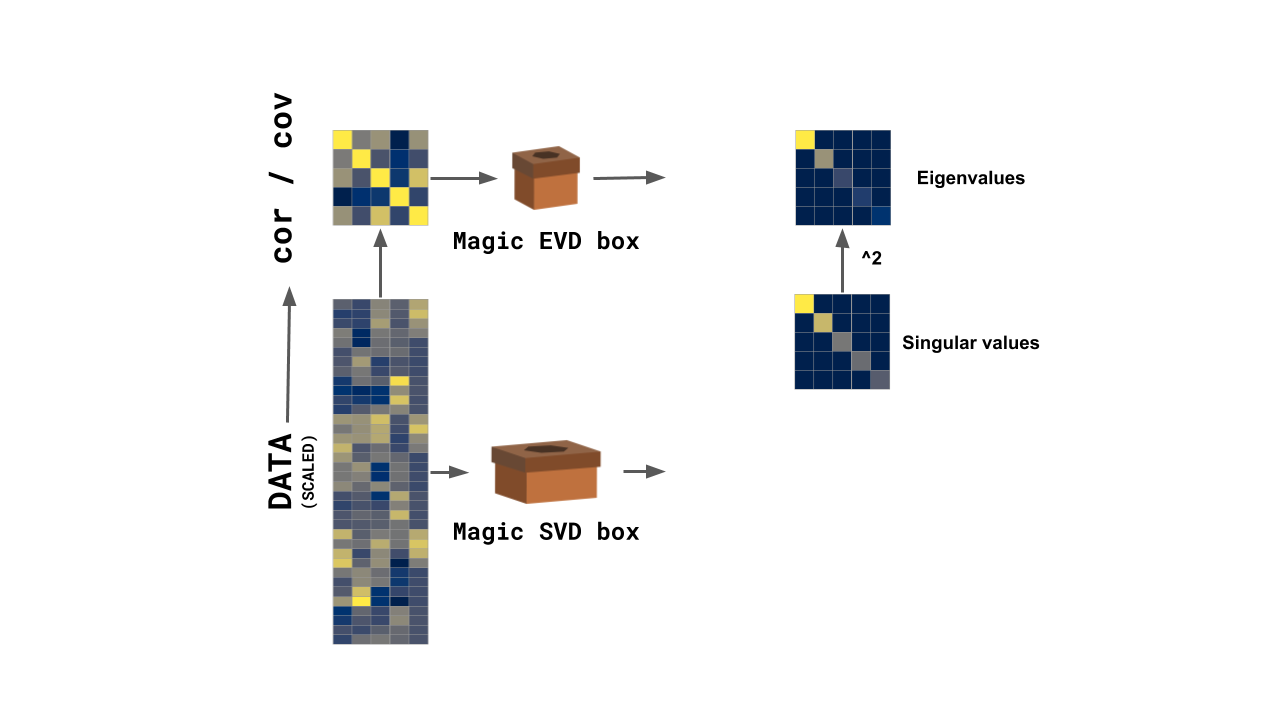
\includegraphics{../images/EVD_SVD_3.png}

\end{frame}

\begin{frame}{Eigen- and singular value decompositions}
\protect\hypertarget{eigen--and-singular-value-decompositions-3}{}

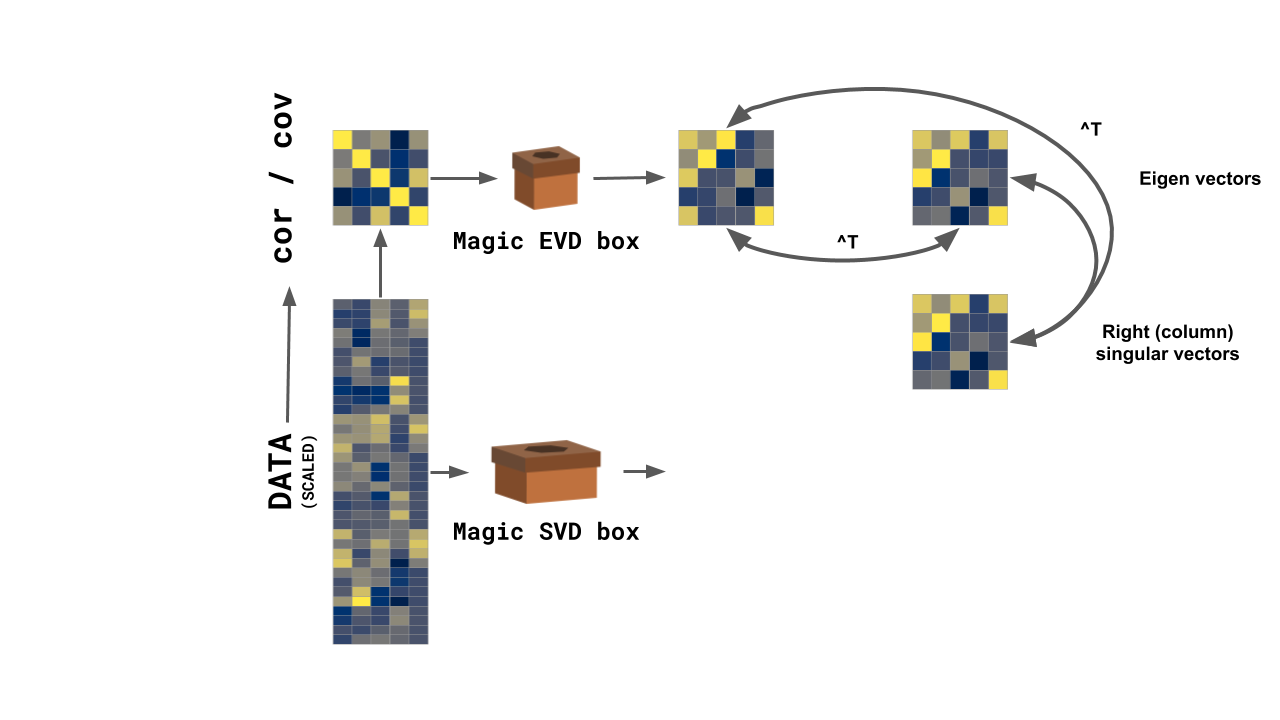
\includegraphics{../images/EVD_SVD_4.png}

\end{frame}

\begin{frame}{Eigen- and singular value decompositions}
\protect\hypertarget{eigen--and-singular-value-decompositions-4}{}

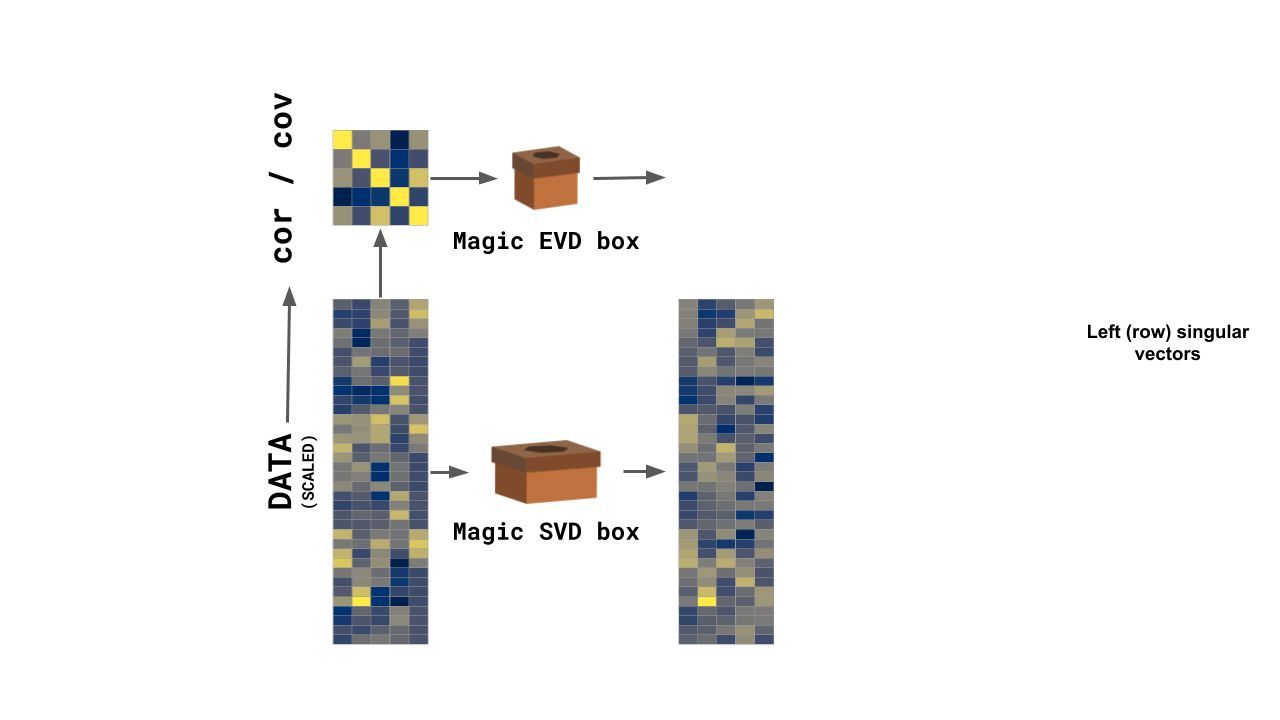
\includegraphics{../images/EVD_SVD_5.png}

\end{frame}

\hypertarget{some-data}{%
\section{Some data}\label{some-data}}

\begin{frame}{Diagnosis and education}
\protect\hypertarget{diagnosis-and-education}{}

\begin{table}[H]
\centering
\begin{tabular}{>{\em}lrrr}
\toprule
  & CN & Dementia & MCI\\
\midrule
ADV & 39 & 7 & 54\\
B & 57 & 17 & 75\\
B+ & 75 & 19 & 113\\
HS & 25 & 13 & 46\\
HS+ & 39 & 9 & 77\\
\bottomrule
\end{tabular}
\end{table}

\end{frame}

\begin{frame}

\begin{itemize}[<+->]
\tightlist
\item
  Given you a table, and asked for a multivariate analysis
\item
  We do what we know: PCA
\end{itemize}

\end{frame}

\begin{frame}

\includegraphics{CA_MCA_Slides_files/figure-beamer/edu_dx_pca_1-1.pdf}

\end{frame}

\begin{frame}{What did we analyze?}
\protect\hypertarget{what-did-we-analyze}{}

\begin{table}[H]
\centering
\begin{tabular}{lrrr}
\toprule
  & CN & Dementia & MCI\\
\midrule
CN & 1.000 & 0.730 & 0.921\\
Dementia & 0.730 & 1.000 & 0.652\\
MCI & 0.921 & 0.652 & 1.000\\
\bottomrule
\end{tabular}
\end{table}

\end{frame}

\begin{frame}{What did PCA detect?}
\protect\hypertarget{what-did-pca-detect}{}

\end{frame}

\begin{frame}{Let's try something different!}
\protect\hypertarget{lets-try-something-different}{}

\begin{table}[H]
\centering
\begin{tabular}{>{\em}lrrrrr}
\toprule
  & ADV & B & B+ & HS & HS+\\
\midrule
CN & 39 & 57 & 75 & 25 & 39\\
Dementia & 7 & 17 & 19 & 13 & 9\\
MCI & 54 & 75 & 113 & 46 & 77\\
\bottomrule
\end{tabular}
\end{table}

\end{frame}

\begin{frame}

\includegraphics{CA_MCA_Slides_files/figure-beamer/edu_dx_pca_2-1.pdf}

\end{frame}

\begin{frame}{What did PCA analyze?}
\protect\hypertarget{what-did-pca-analyze}{}

\begin{table}[H]
\centering
\begin{tabular}{lrrrrr}
\toprule
  & ADV & B & B+ & HS & HS+\\
\midrule
ADV & 1.000 & 1.000 & 0.995 & 0.935 & 0.963\\
B & 1.000 & 1.000 & 0.994 & 0.932 & 0.960\\
B+ & 0.995 & 0.994 & 1.000 & 0.965 & 0.984\\
HS & 0.935 & 0.932 & 0.965 & 1.000 & 0.996\\
HS+ & 0.963 & 0.960 & 0.984 & 0.996 & 1.000\\
\bottomrule
\end{tabular}
\end{table}

\end{frame}

\begin{frame}{What did PCA detect?}
\protect\hypertarget{what-did-pca-detect-1}{}

\begin{table}[H]
\centering
\begin{tabular}{>{\em}lrrrrr>{\bfseries}r}
\toprule
  & ADV & B & B+ & HS & HS+ & Row sums\\
\midrule
CN & 39 & 57 & 75 & 25 & 39 & 235\\
Dementia & 7 & 17 & 19 & 13 & 9 & 65\\
MCI & 54 & 75 & 113 & 46 & 77 & 365\\
\bottomrule
\end{tabular}
\end{table}

\end{frame}

\begin{frame}{What is PCA for?}
\protect\hypertarget{what-is-pca-for-1}{}

\begin{itemize}[<+->]
\tightlist
\item
  When we can compute a \emph{meaningful} covariance or correlation
  matrix
\end{itemize}

\end{frame}

\begin{frame}[fragile]{Let's take another look}
\protect\hypertarget{lets-take-another-look}{}

\begin{verbatim}
## Warning in rbind(cbind(edu_dx_table, rowSums(edu_dx_table)),
## colSums(edu_dx_table)): number of columns of result is not a multiple of
## vector length (arg 2)
\end{verbatim}

NA

\end{frame}

\hypertarget{simple-correspondence-analysis}{%
\section{Simple correspondence
analysis}\label{simple-correspondence-analysis}}

\begin{frame}{History}
\protect\hypertarget{history}{}

\begin{itemize}[<+->]
\tightlist
\item
  CA

  \begin{itemize}[<+->]
  \tightlist
  \item
    Hirschfeld (1935)
  \item
    Guttman (1941)
  \item
    Burt (1950)
  \item
    Benzecri (1964)
  \item
    Escofier (1965)
  \end{itemize}
\item
  See Lebart's History \& Prehistory of CA:
  \url{http://www.dtmvic.com/doc/About_the_History_of_CA.pdf}
\end{itemize}

\end{frame}

\begin{frame}{Chi-squared}
\protect\hypertarget{chi-squared}{}

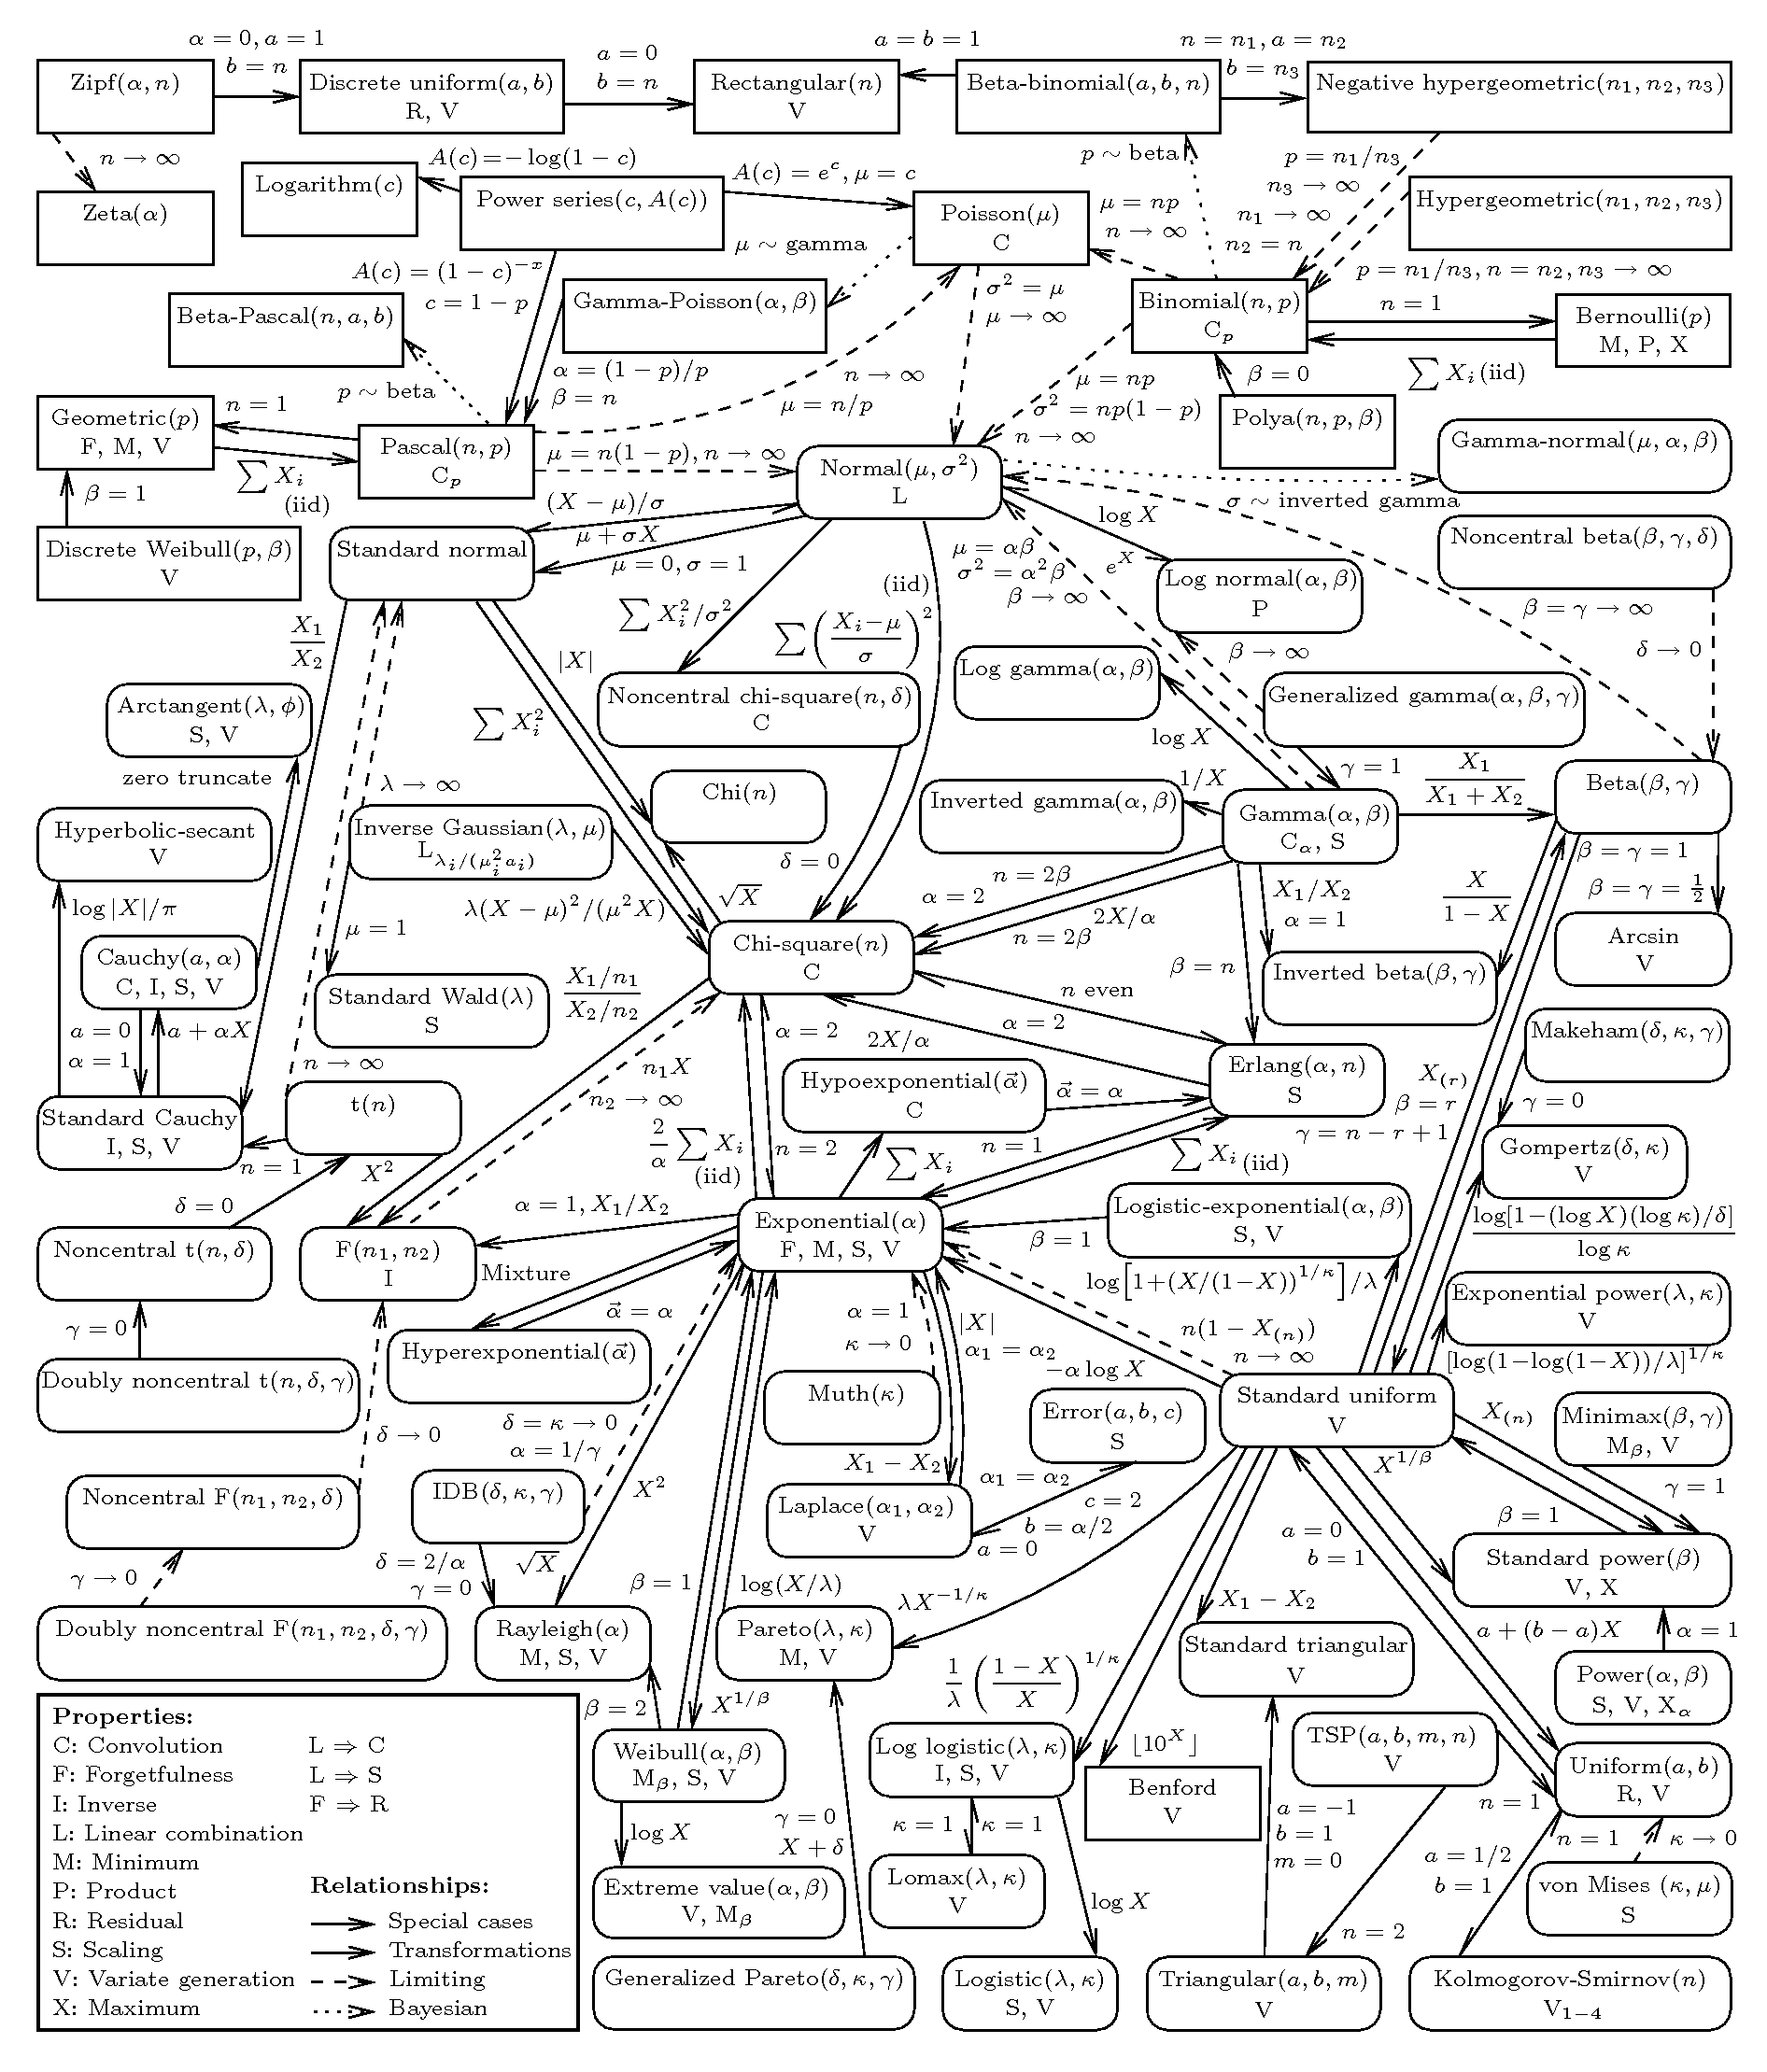
\includegraphics{../images/distributions.png}

\href{http://www.math.wm.edu/~leemis/chart/UDR/UDR.html}{See here}

\end{frame}

\begin{frame}{Chi-squared}
\protect\hypertarget{chi-squared-1}{}

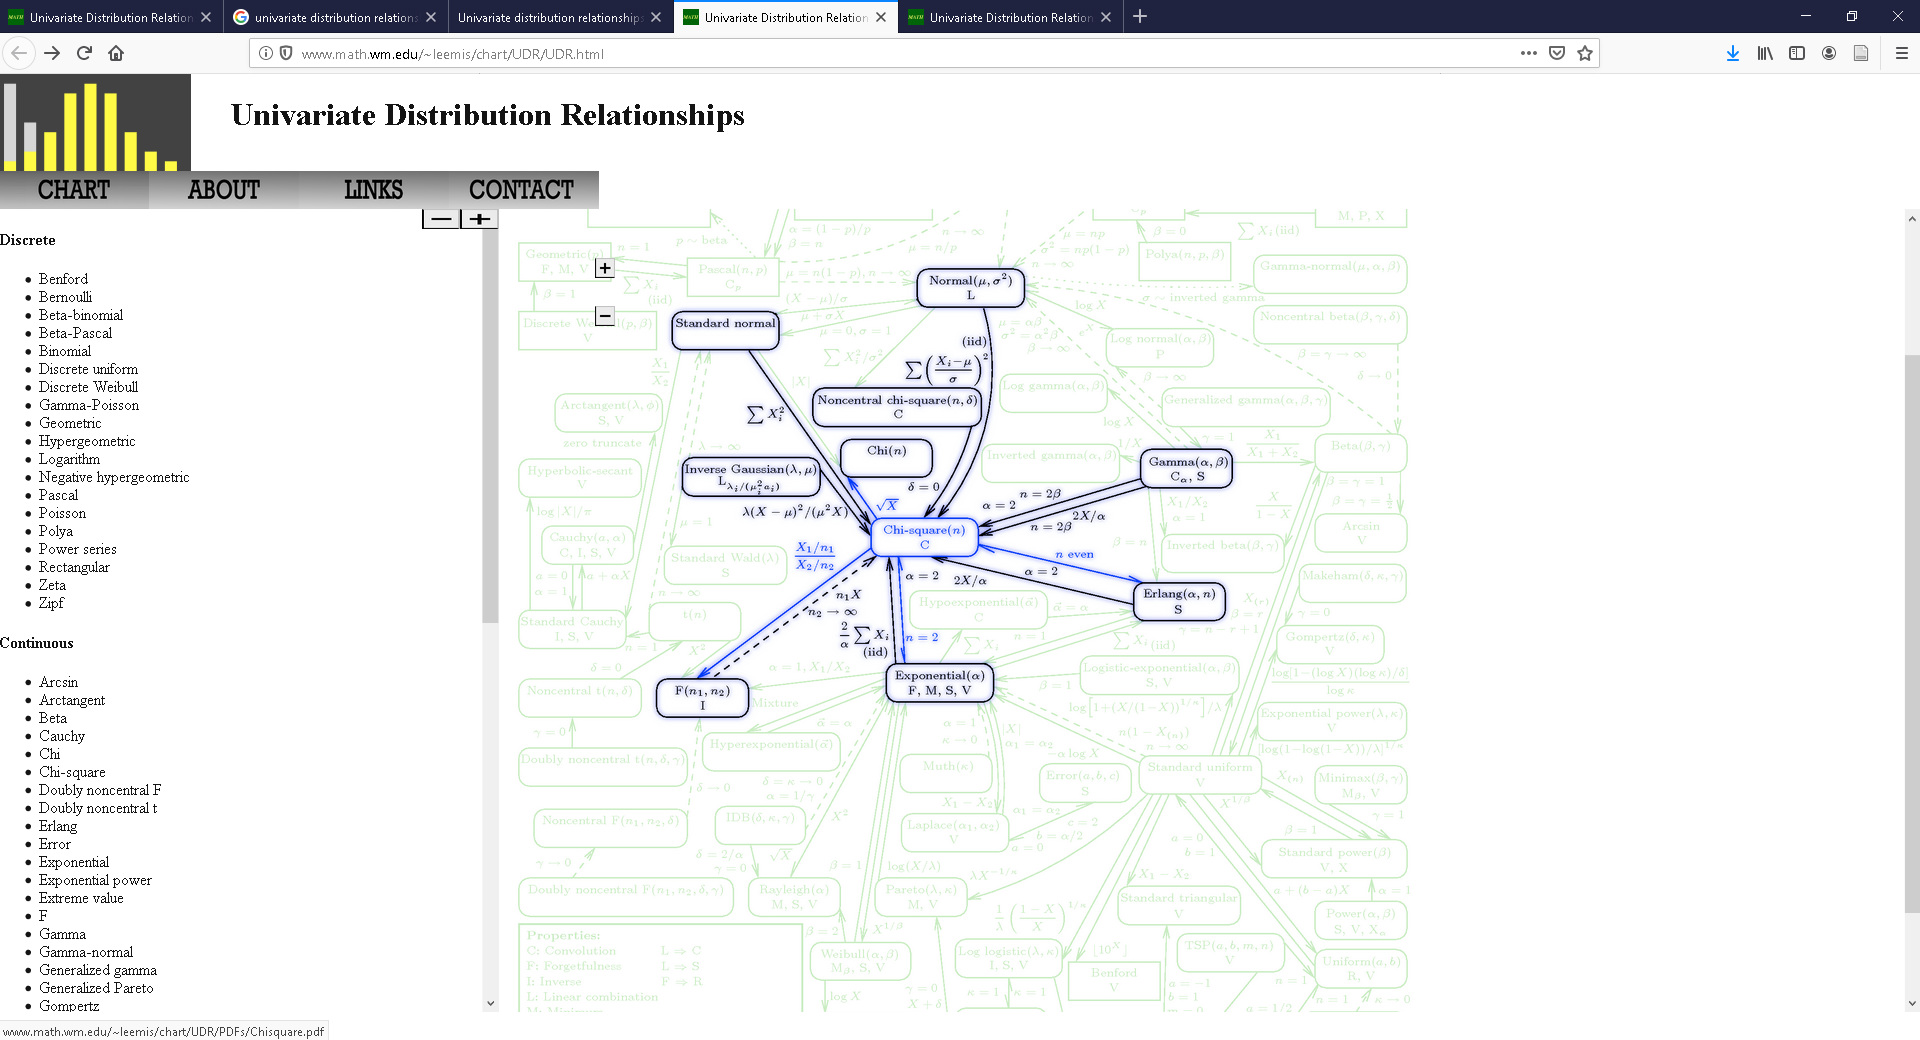
\includegraphics{../images/Chi2.PNG}

\href{http://www.math.wm.edu/~leemis/chart/UDR/UDR.html}{See here}

\end{frame}

\begin{frame}{Under the hood}
\protect\hypertarget{under-the-hood}{}

\begin{itemize}[<+->]
\tightlist
\item
  The eigenvalue decomposition (EVD)

  \begin{itemize}[<+->]
  \tightlist
  \item
    Requires squares, symmetric, and positive semi definite
  \item
    Generally correlation or covariance
  \end{itemize}
\item
  The singular value decomposition (SVD)

  \begin{itemize}[<+->]
  \tightlist
  \item
    Works with rectangular tables
  \end{itemize}
\item
  The generalized SVD

  \begin{itemize}[<+->]
  \tightlist
  \item
    Apply constraints (weights) to rows \& columns of rectangular table
  \item
    Required for CA and fancier PCA-like techniques \& extensions
  \end{itemize}
\end{itemize}

\end{frame}

\begin{frame}{The GSVD}
\protect\hypertarget{the-gsvd}{}

\end{frame}

\hypertarget{multiple-correspondence-analysis}{%
\section{Multiple correspondence
analysis}\label{multiple-correspondence-analysis}}

\hypertarget{some-many-bonuses}{%
\section{Some many bonuses!}\label{some-many-bonuses}}

\hypertarget{software}{%
\subsection{Software}\label{software}}

\begin{itemize}[<+->]
\tightlist
\item
  ExPosition

  \begin{itemize}[<+->]
  \tightlist
  \item
    Family of packages
  \item
    Includes resampling
  \item
    Lots of PCA \& CA techniques
  \end{itemize}
\item
  factoextra

  \begin{itemize}[<+->]
  \tightlist
  \item
    Awesome ggplot2 visualizers for ExPosition
  \item
    \url{http://www.alboukadel.com/} \&
    \url{http://www.sthda.com/english/}
  \end{itemize}
\item
  ours

  \begin{itemize}[<+->]
  \tightlist
  \item
    Developed here within ONDRI
  \item
    New package for outliers
  \item
    Has some important bells-and-whistles
  \end{itemize}
\end{itemize}

\hypertarget{some-alternatives}{%
\subsection{Some alternatives}\label{some-alternatives}}

\begin{itemize}[<+->]
\tightlist
\item
  FactoMineR
\item
  ade4
\item
  ca
\item
  MASS
\item
  psych
\item
  So many others
\end{itemize}

\hypertarget{some-references}{%
\section{(Some) References}\label{some-references}}

\begin{frame}{See the reference sections of these}
\protect\hypertarget{see-the-reference-sections-of-these}{}

\begin{itemize}[<+->]
\item
  Beaton, D., Saporta, G., Abdi, H., \& Alzheimer's Disease Neuroimaging
  Initiative. (2019). A generalization of partial least squares
  regression and correspondence analysis for categorical and mixed data:
  An application with the ADNI data. bioRxiv, 598888.
\item
  Beaton, D., Sunderland, K. M., Levine, B., Mandzia, J., Masellis, M.,
  Swartz, R. H., \ldots{} \& Strother, S. C. (2019). Generalization of
  the minimum covariance determinant algorithm for categorical and mixed
  data types. bioRxiv, 333005.
\end{itemize}

\end{frame}

\begin{frame}{And these}
\protect\hypertarget{and-these}{}

\begin{itemize}[<+->]
\item
  Abdi, H., Guillemot, V., Eslami, A., \& Beaton, D. (2017). Canonical
  correlation analysis. Encyclopedia of Social Network Analysis and
  Mining, 1-16.
\item
  Beaton, D., Dunlop, J., \& Abdi, H. (2016). Partial least squares
  correspondence analysis: A framework to simultaneously analyze
  behavioral and genetic data. Psychological methods, 21(4), 621.
\end{itemize}

\end{frame}

\begin{frame}{Techniques}
\protect\hypertarget{techniques}{}

\begin{itemize}[<+->]
\item
  Greenacre, M. (2017). Correspondence analysis in practice. CRC press.
\item
  Greenacre, M. J. (1984). Theory and Applications of Correspondence
  Analysis. Retrieved from
  \url{http://books.google.com/books?id=LsPaAAAAMAAJ}
\end{itemize}

\end{frame}

\begin{frame}{Techniques}
\protect\hypertarget{techniques-1}{}

\begin{itemize}[<+->]
\item
  Greenacre, M. J. (2010). Correspondence analysis. Wiley
  Interdisciplinary Reviews: Computational Statistics, 2(5), 613--619.
  \url{https://doi.org/10.1002/wics.114}
\item
  Lebart, L., Morineau, A., \& Warwick, K. M. (1984). Multivariate
  descriptive statistical analysis: correspondence analysis and related
  techniques for large matrices. Wiley.
\item
  Nguyen, L. H., \& Holmes, S. (2019). Ten quick tips for effective
  dimensionality reduction. PLOS Computational Biology, 15(6), e1006907.
\end{itemize}

\end{frame}

\begin{frame}{Data}
\protect\hypertarget{data}{}

\begin{itemize}[<+->]
\item
  Escofier, B. (1978). Analyse factorielle et distances répondant au
  principe d'équivalence distributionnelle. Revue de Statistique
  Appliquée, 26(4), 29--37.
\item
  Escofier, B. (1979). Traitement simultané de variables qualitatives et
  quantitatives en analyse factorielle. Cahiers de l'Analyse Des
  Données, 4(2), 137--146.
\item
  Greenacre, M. (2014). Data Doubling and Fuzzy Coding. In J. Blasius \&
  M. Greenacre (Eds.), Visualization and Verbalization of Data
  (pp.~239--253). Philadelphia, PA, USA: CRC Press.
\end{itemize}

\end{frame}

\end{document}
